%!TEX TS-program = XeLaTeX
\documentclass[11pt]{article}

\usepackage{amssymb}
\usepackage{amsthm}
\usepackage{amsmath}
\usepackage{mathtools}

\usepackage{fancyhdr}
\usepackage{graphicx}
\usepackage[top=3cm, left=2cm, right=2cm, headheight = 90pt]{geometry}
\usepackage{xltxtra}
\usepackage[font=small,labelfont=bf]{caption}

%%%%%%%%%%%%%%    Language matters  %%%%

%\usepackage[latvian]{babel}
%\usepackage[L7x]{fontenc}
%\usepackage[utf8x]{inputenc}

%%%%%%%%%%%%%%%%%%%%%%%%%%%%%%%%%%%7%%%%%

%%%%%%%%%%%%%%%%%%%%%%%%%%%       DO NOT EDIT         %%%%%%%%%%%%%%%%%%
%\usepackage{space}
%\renewcommand{\headrulewidth}{1pt}
%\fancyhead[L]{\includegraphics[width=3cm]{pictures/logo}}
%\fancyhead[R]{\raisebox{3ex}{\fbox{Language: \bf \lang}}}
\fancyhead[C]{{\Large\bf Strategies and tactics - Problems}\\ \date}

\renewcommand{\theenumi}{\alph{enumi}}
%\newcommand{\problem}[1]{\paragraph{Problem #1.}}%<--------------- TRANSLATE THE WORD "Problem".
\fancyfoot[CE,CO]{}  % this is to remove page numbers (as you might want for single page docs)

\def\leq{\leqslant}
\def\geq{\geqslant}
\def\N{\mathbb N}
\def\R{\mathbb R}
\def\Z{\mathbb Z}
\DeclarePairedDelimiter\set\{\}

%%%%%%%%%%%%%%%%%%%%%%%%%%%%%%%%%%%%%%%%%%%%%%%%%%%%%%%%%%%%%%%%%%%%%%%%%


%%% Language name in english %%%%%%%%%
\def\lang{Latvian}

%\def\lang{Lithuanian}

%%%%%%%%%%%%%%%%%%%%%%%%%%%%% TRANSLATE HERE %%%%%%%%%%%%%%%%%%%%%%%%%%%%%%%%%%

%\def\date{2018. gada 18. jūnijs}
%\def\notes{}


%%%%%%%%%%%%%%%%%%%%%%%%%%%%%%%%%%%%%%%%%%%%%%%%%%%%%%%%%%%%%%%%%%%%%%%%%%%%%%%

\def\prob{}

%%%%%%%%%%%%%%%%%%%%%%%%%%%%%%%%%%%%%%%%%%%%%%%%%%%%%%%%

\theoremstyle{definition}
\newtheorem{problem}{\prob}

\pagestyle{fancy}



\begin{document}
%\thispagestyle{fancy}
\noindent 
%\emph{\notes}

%1
\begin{problem}
\textit{[Bridge problem - "expanding a problem"]}
Its a dark night and four men are fleeing from terrible danger and must cross a ravine where only way across is a long narrow bridge. Only two people can be on the bridge at the same time. It's also very dark and they have only one lantern with them. Lantern is not very strong, so to be on a bridge, a person must be right next to a lantern (so, one or two people can cross carrying a lantern). 
People are different - one of them is fast and can cross a bridge in $1$ minute, other is a bit slower - $2$ minutes, third is even slower and takes $5$ minutes and last one takes $10$ minutes to cross.
If all of that were not enough the bridge is rigged and will explode in exactly $18$ minutes. 

Can all four make it across?
\begin{center}
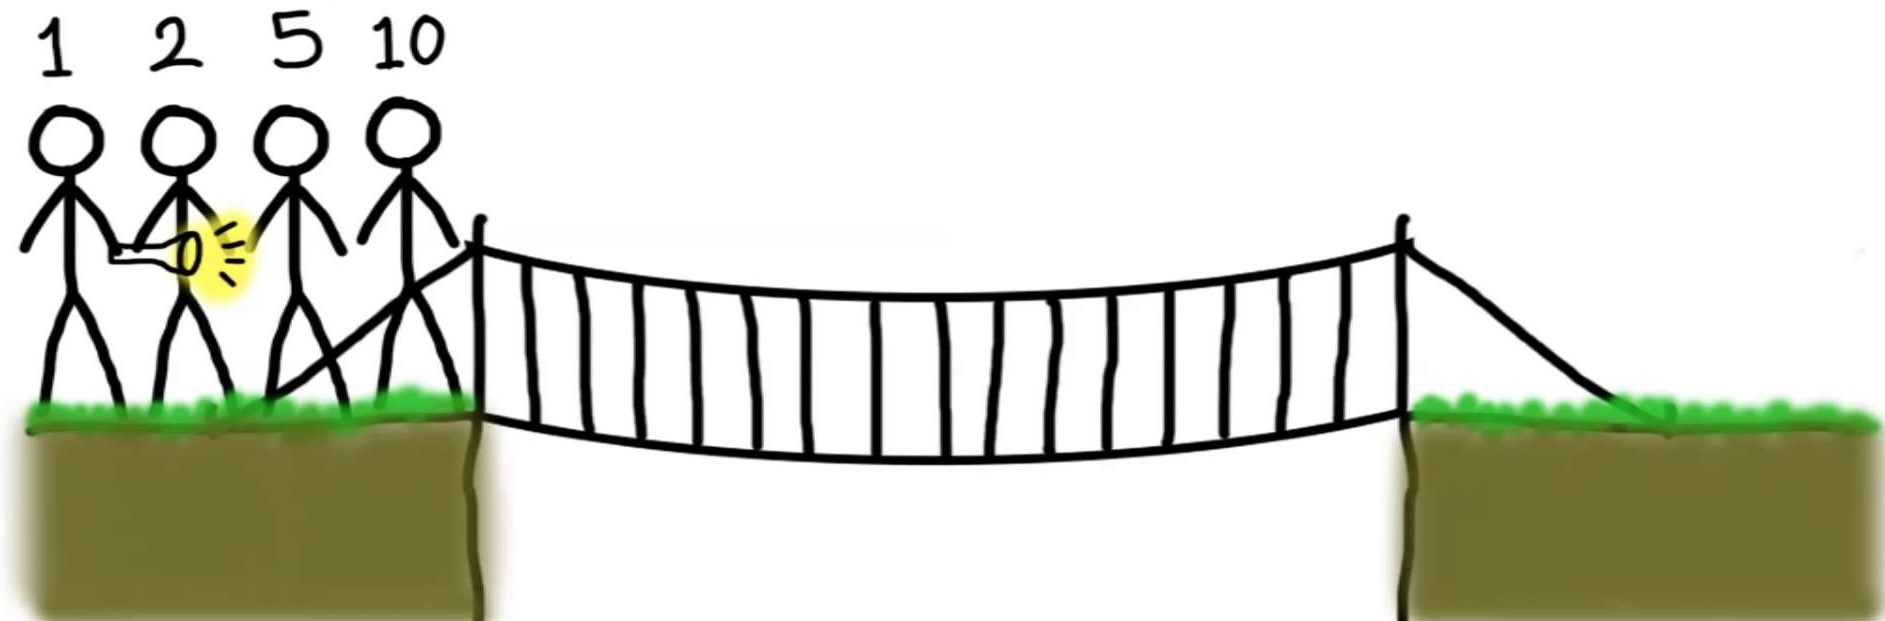
\includegraphics[width=5cm]{bridge.jpg}
\captionof{figure}{Crossing a narrow bridge}
\label{fig:bridge}
\end{center}
\end{problem}
%

%2
\begin{problem}
\textit{[9 dots - "thinking outside the box"]}
$9$ dots are drawn in a $3 \times 3$ grid on a piece of paper. Can you draw $4$ straight, continuous lines that connect all the dots, without lifting the pencil from the paper?
\begin{center}

\includegraphics[width=2cm]{3by3.jpg}
\captionof{figure}{9 dots}
\label{fig:bridge}
\end{center}
\end{problem}
%

%3
\begin{problem}
\textit{[More dots - "reduction","thinking outside the box"]}
Same as previous problem, but with:
\begin{enumerate}
\item $5 \times 5$ with $8$ lines 
\item $4 \times 4$ with $6$ lines
\item $3 \times 4$ with $5$ lines
\item $4 \times 5$ with $7$ lines
\end{enumerate}
\end{problem}
%

%4
\begin{problem}
\textit{[Sultan's law - "symmetry"]}
There is equal amount of men and women in Arabia, but, for religious reasons, Sultan would wish it that there would be more women than men. 

He decides on the following law: each couple has to keep having children until a first son is born and then stop having children. How well would this law work? What would be the average size of family with this law?
\end{problem}
%


%5
\begin{problem}
\textit{[Gambling problem - "symmetry"]}
Elize and Rudolf were bored during a class and decided to play a gambling game. They have a fair coin, but instead of keeping it simple they decided on a following game: first each of them chose a $3$ event string (for example "heads-heads-tails"). Then they start tossing a coin and write down results until they encounter one of the chosen substrings, which then is the winner. Decide if the game is fair for the following:
\begin{enumerate}
\item "heads-heads-heads" vs "tails-tails-tails"
\item "heads-heads-heads" vs "heads-heads-tails"
\item "tails-tails-heads" vs "heads-heads-tails"
\item "tails-tails-heads" vs "heads-heads-heads"
\end{enumerate}

\end{problem}
%
\end{document}
